\documentclass[12pt,a4paper, twosite]{article}
\usepackage{mystyle}

%oben und unten
\usepackage{fancyhdr}
\pagestyle{fancy}
\lhead{St. Michael\\Fribourg}
\rhead{Labor: Radioaktivität}
\rfoot{Felix Binder}
\lfoot{Januar 2014}
\renewcommand\headrulewidth{1pt}
\renewcommand\footrulewidth{1pt}
%ende oben und unten


\author{}
\date{}
\title{Radioaktivität}

\begin{document}
\maketitle
%\thispagestyle{empty}
%\section*{Ablauf}
%Das Labor zur Kernphysik/Radioaktivität findet über zwei Termine statt. 
%Jede Gruppe bekommt ein eigenes Thema, und bearbeitet dies selbstständig.
%Während des ersten Termins müssen alle Messungen durchgeführt werden. 
%Der zweite Termin ist für die Präsentation der eigenen Arbeit reserviert.
%Jede Präsentation sollte etwa 12 bis \SI{15}{Minuten} dauern.

\section*{Sicherheitshinweise}
Während des Labors wird mit schwach radioaktiven Stoffen gearbeitet. Diese haben richtig angewendet keinen Einfluss auf
die Gesundheit. Das Labormaterial im Speziellen das Geiger-Müller-Zählrohr sind sehr empfindlich.
Bei nicht Benutzung ist stets der Plastikschutz aufzustecken. Die Membran ist sehr dünn und darf niemals berührt werden.
Die Kosten bei Neubeschaffung sind sehr hoch (800 Fr.).

\section*{Material}
Für diesen Praktikumsversuch werden folgende Materialien benötigt:
\begin{itemize}
	\item Experimentierkasten Radioaktivität 
	\item Geiger-Müller-Zählrohr
	\item Computer für die Recherche und die Erstellung einer Präsentation und eines Laborberichtes.
\end{itemize}

\section*{Vorbereitung und Versuchsaufbau}

\textbf{Nullmessung:}
Ist eine Messung in Abwesenheit des zu messenden Effekts.
Bei Strahlungsmessungen stellt man zunächst mit einer Nullmessung fest, 
wie hoch der Strahlungsuntergrund im Messraum und der Eigennulleffekt des Messgerätes sind.
Aufgrund der geringen Aktivität ist bei kurzen Messzeiten mit einer grossen Messungenauigkeit zu rechnen.
Tipp: Halten Sie bei allen Messungen die Messgenauigkeit jederzeit im Blick!

Eine Tabelle für die Nullmessung könnte so aussehen:

\usetikzlibrary{matrix}
\tikzset{ 
    table/.style={
        matrix of nodes,
        row sep=-\pgflinewidth,
        column sep=-\pgflinewidth,
        nodes={
            rectangle,
            draw=black,
            align=center
        },
        minimum height=1.5em,
        text depth=0.5ex,
        text height=2ex,
        nodes in empty cells,
%%
        every even row/.style={
            nodes={fill=gray!20}
        },
        column 1/.style={
            nodes={text width=7em,font=\bfseries}
        },
        row 1/.style={
            nodes={
             %   fill=black,
             %   text=white,
                font=\bfseries
            }
        }
    }
}

\begin{tikzpicture}

\matrix (first) [table,text width=10em]
{
Zeit $t$ (min) & Impulse $N$   & {Zählrate $n$ ($s^{-1}$)} \\
2   &   &            \\
4   &   &            \\
6   &   &            \\
8   &   &            \\
10   &   &            \\
12   &   &            \\
14   &   &            \\
16   &   &            \\
18   &   &            \\
20   &   &            \\
};

\end{tikzpicture}

Die Zählrate $n$ bestimmt sich aus den gemessenen Impulsen pro Zeit.
Aufgrund des statistischen Charakters der Radioaktivität schwankt der Wert der Zählrate. Die Zählrate sollte sich aber mit der Zeit einem
festen Wert annähern. Sind sie mit der Genauigkeit von $n$ zufrieden, können Sie die Nullmessung beenden.

\section*{Paranuss}
Die Aktivität der Paranuss ist nicht sehr hoch, daher sollte man versuchen, durch lange Messzeiten 
eine akzeptable Messgenauigkeit zu erreichen. Der Schwerpunkt dieses Projektes liegt nicht so sehr in
der Durchführung von vielen verschiedenen Messungen, sondern eher in der Recherche und Einordnung der Messergebnisse. 

Mögliche Fragestellungen sind:
\begin{itemize}
	\item Warum ist die Paranuss radioaktiv?
	\item Was ist für diese radioaktive Strahlung verantwortlich?
	\item Ist es gesundheitsgefährlich Paranüsse zu essen? Und wenn, wie viele darf man bedenkenlos essen?
	\item Gibt es noch andere radioaktive Lebensmittel?
	\item Wo kommt Radioaktivität sonst noch vor?
\end{itemize}



\newpage

\section*{Kaliumsulfat}
Kaliumsulfat ist das Kaliumsalz der Schwefelsäure. Es wird hauptsächlich als Düngemittel verwendet, kommt aber auch
in kleinen Mengen als Lebensmittelzusatz E515 zum Einsatz.
Die Aktivität von Kaliumsulfat ist nicht sehr hoch, daher sollte man versuchen, durch lange Messzeiten 
eine akzeptable Messgenauigkeit zu erreichen. Der Schwerpunkt dieses Projektes liegt nicht so sehr in
der Durchführung von vielen verschiedenen Messungen, sondern eher in der Recherche und Einordnung der Messergebnisse. 

Mögliche Fragestellungen sind:
\begin{itemize}
	\item Warum ist Kaliumsulfat radioaktiv?
	\item Was ist für diese radioaktive Strahlung verantwortlich?
	\item Ist es gesundheitsgefährlich? Und wenn, wie viel darf man bedenkenlos zu sich nehmen? 
	\item Gibt es noch andere radioaktive Lebensmittel?
	\item Wo kommt Radioaktivität sonst noch vor?
\end{itemize}
\newpage

\section*{Winkelabhängigkeit radioaktiver Strahlung}
Dieses Projekt ist mit vielen Einzelmessungen verbunden. Wählen Sie eine Strahlungsquelle mit möglichst hoher
Aktivität. Die einzelnen Winkelstellungen, die sie untersuchen werden weisen unterschiedliche Zählraten auf.

Tipp: Führen Sie winkelabhängige Messungen mit und ohne Magnete durch.

Mögliche Fragestellungen sind:
\begin{itemize}
	\item Warum werden radioaktiven Strahlen vom Magnetfeld abgelenkt?
	\item Können Sie die Zusammensetzung der Strahlung bestimmen?
	\item Lässt sich damit auf das Alter der Probe schliessen?
\end{itemize}

\begin{figure}[t]
	\begin{center}
	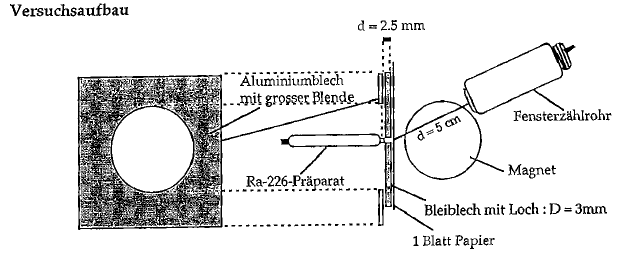
\includegraphics{winkel1.png}
	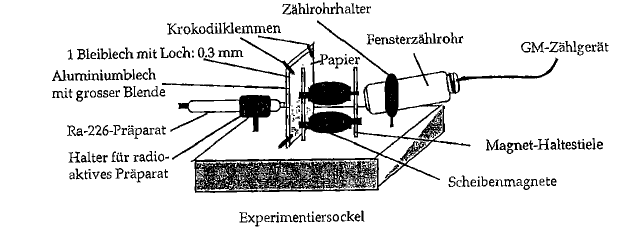
\includegraphics{winkel2.png}
%	\caption{Skizze des Versuchsaufbaus.} 
	\end{center}
\end{figure}
\newpage

\section*{Abschirmung von radioaktiver Strahlung}
Dieses Projekt ist mit vielen Einzelmessungen verbunden. Wählen Sie eine Strahlungsquelle mit möglichst hoher
Aktivität. Benutzen Sie unterschiedliche Materialien, um die radioaktive Strahlung der Quelle abzuschirmen. 

Mögliche Fragestellungen sind:
\begin{itemize}
	\item Warum lassen sich radioaktive Strahlen abschirmen?
	\item Welche Strahlung braucht welches Material zum abschirmen?
	\item Was ist die Halbwertsdicke?
	\item Kann man die Probe durch Abschirmung charakterisieren?
	\item Lässt sich damit auf das Alter der Probe schliessen?
\end{itemize}

\end{document}
